\chapter{Tutorial on using SPREAD software}

% \begin{flushleft}
% \textbf{Authors}
% \par\end{flushleft}
% 
% \noindent
% Filip Bielejec (\url{filip.bielejec(sorry_spybots)rega.kuleuven.be}) \\
% Philippe Lemey (\url{philippe.lemey(sorry_spybots)rega.kuleuven.be}) \\
% Andrew Rambaut (\url{a.rambaut(sorry_spybots)ed.ac.uk}) \\
% Marc Suchard (\url{msuchard(sorry_spybots)ucla.edu})\\

\begin{flushleft}
\textbf{Download}
\par\end{flushleft}
Compiled, runnable program can be downloaded from: \url{http://www.phylogeography.org/SPREAD.html}
Get the source code on GitHub: \url{https://github.com/phylogeography/SPREAD}.
You can also clone the project with Git by running:

\begin{lyxcode}
git~clone~git@github.com:phylogeography/SPREAD.git
\end{lyxcode}
% \pagebreak{}

\section{Introduction}

In this supplement we give a detailed description of program functionalities, describe some possible analysis and give general guidelines on running Spread. 
We present an example for each of the possible analysis. 
The example files used in the analysis can be accessed from \url{http://www.phylogeography.org/SPREAD.html}.
The generated visualisations can be opened for viewing in Google Earth (\url{www.google.com/earth/}) or any other GIS software capable of reading the Keyhole Markup Language (KML) format.


\section{Recommended platform, hardware and software for Spread}

Spread will run on a variety of platforms, as long as a suitable Java
Runtime Environment is present. Recommended JRE include OpenJDK and
Sun JRE, however application will also run on other runtime environments.
Spread has been tested on well established operating systems namely
Debian GNU/Linux, Mac OS X, Windows XP, as well as more esoteric ones
like Nokia Linux Maemo 5 and Linux MeeGo. For most of the templates
following hardware is sufficient: 

\begin{itemize}
\item CPU: Intel CPU 600 MHz or above
\item Main Memory: 1 GB or above
\item Runtime Environment: Sun Java Runtime Environment or OpenJDK 
\end{itemize}
The Time Slicer analysis is more resource-hungry and therefore we
recommend running it with following hardware:
\begin{itemize}
\item CPU: Intel Core 2 Duo 2.0 Ghz or above
\item Main Memory: 3 GB or above
\item Runtime Environment: Sun Java Runtime Environment or OpenJDK 
\end{itemize}

\section{Visualizing location annotated MCC tree}

This tutorial assumes the user has generated the location annotated
Maximum Clade Credibility (MCC) tree. 
Good tutorial on doing so can be found in Tree Summary section of BEASTs tutorial wiki: 

\url{http://beast.bio.ed.ac.uk/Tree_summary} 

\noindent
The example tree file and location coordinates file for this analysis can be found here:

\url{http://www.kuleuven.be/aidslab/phylogeography/SPREAD_files/H5N1_HA_discrete_MCC.tre}

\noindent
and here: 

\url{http://www.kuleuven.be/aidslab/phylogeography/SPREAD_files/locationCoordinates_H5N1.txt}

\noindent
This example considers influenza A H5N1 diffusion among 7 discrete locations. 
We will visualise this data using Spread own map and virtual globe software. 


\subsection{Loading the data}

Click on the Discrete Model tab, then on the Load tree file button
and navigate to the location of your MCC tree file to load it.

\begin{figure}[H]
\begin{centering}
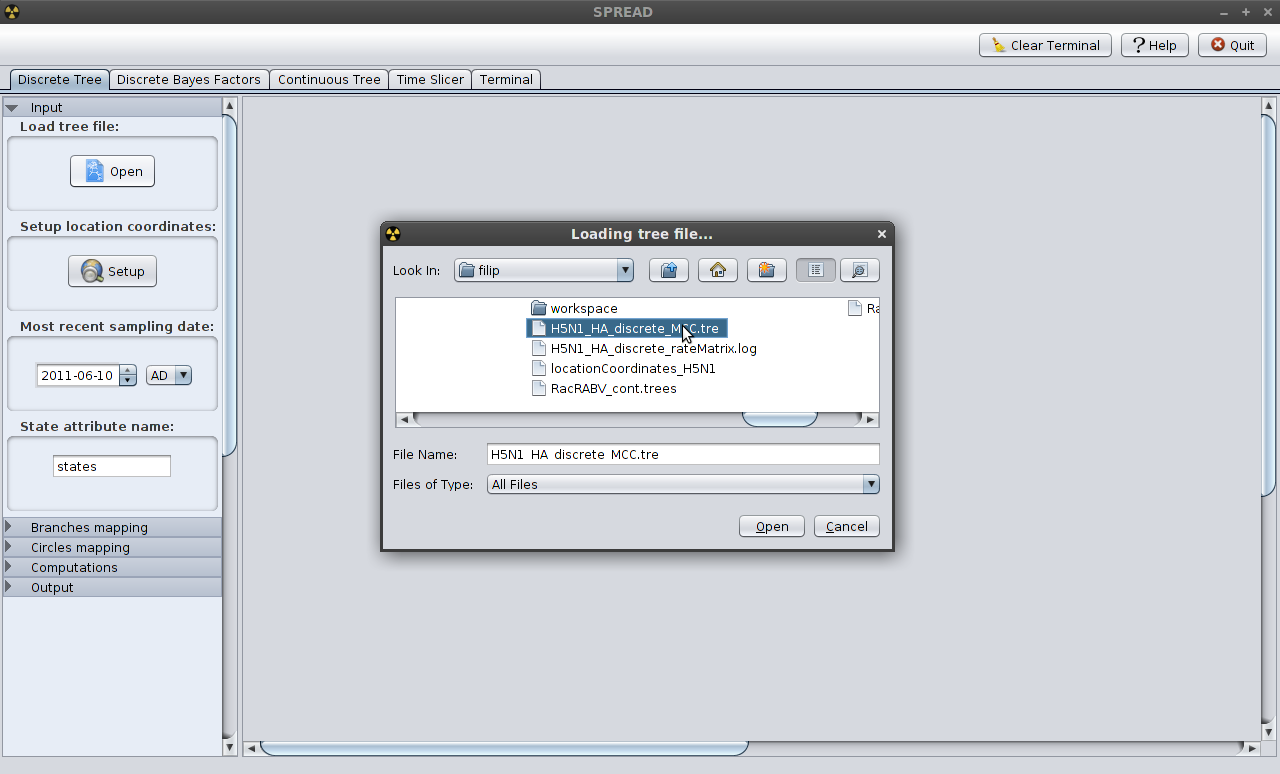
\includegraphics[scale=0.25]{fig01}
\par\end{centering}
\caption{Loading MCC tree file.}
\label{fig:01}
\end{figure}


The Spread will now set the working directory to the one containing
your file. This means that the generated KML output will be saved
in that directory.

\begin{figure}[H]
\begin{centering}
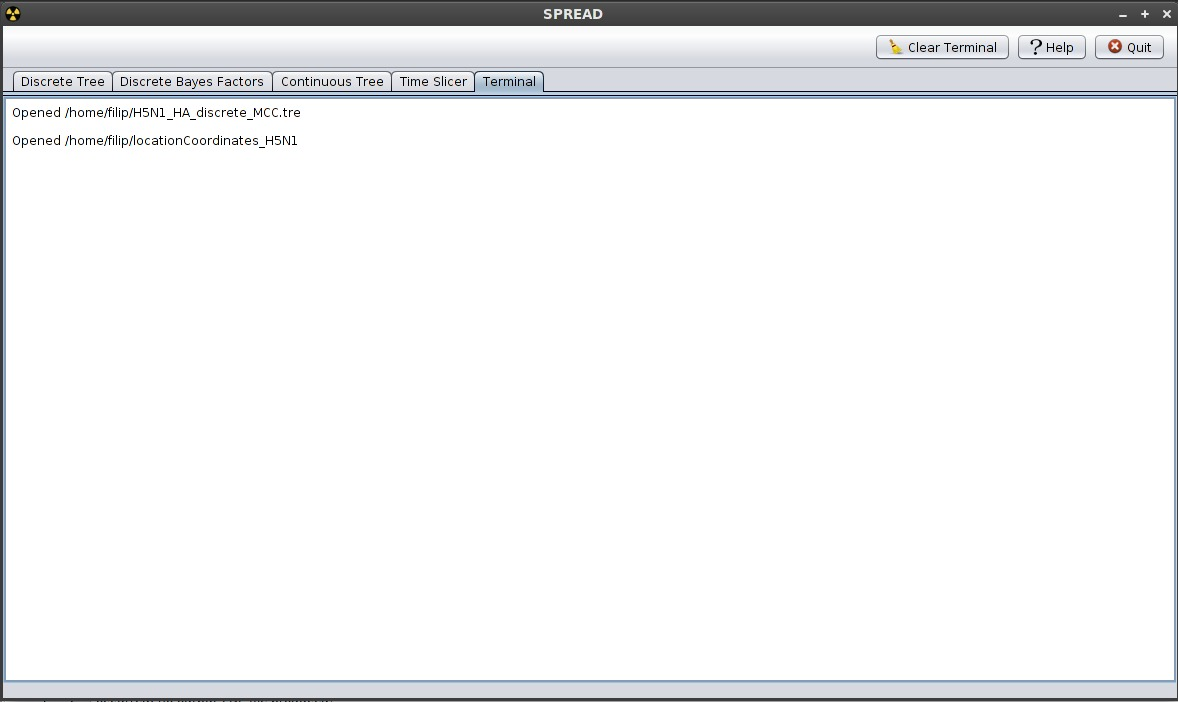
\includegraphics[scale=0.25]{fig02}
\caption{Message in Terminal.}
\label{fig:02}
\par\end{centering}
\end{figure}


To view the MCC tree in it's geographic context, we have to associate
each location with a particular latitude and longitude. To this purpose,
you can either use the editor supplied with Spread and generate the
input file or load previously prepared tab-delimited file including
each location, its latitude and longitude. For the H5N1 example, the
file should look like this:

\begin{lyxcode}
% \centering
Fujian~25.917~118.283

Guangdong~22.87~113.483

Guangxi~23.6417~108.1

Hebei~39.3583~116.6417

Henan~33.875~113.5

HongKong~22.3~114.167

Hunan~27.383~111.517
\end{lyxcode}

\begin{figure}[H]
\begin{centering}
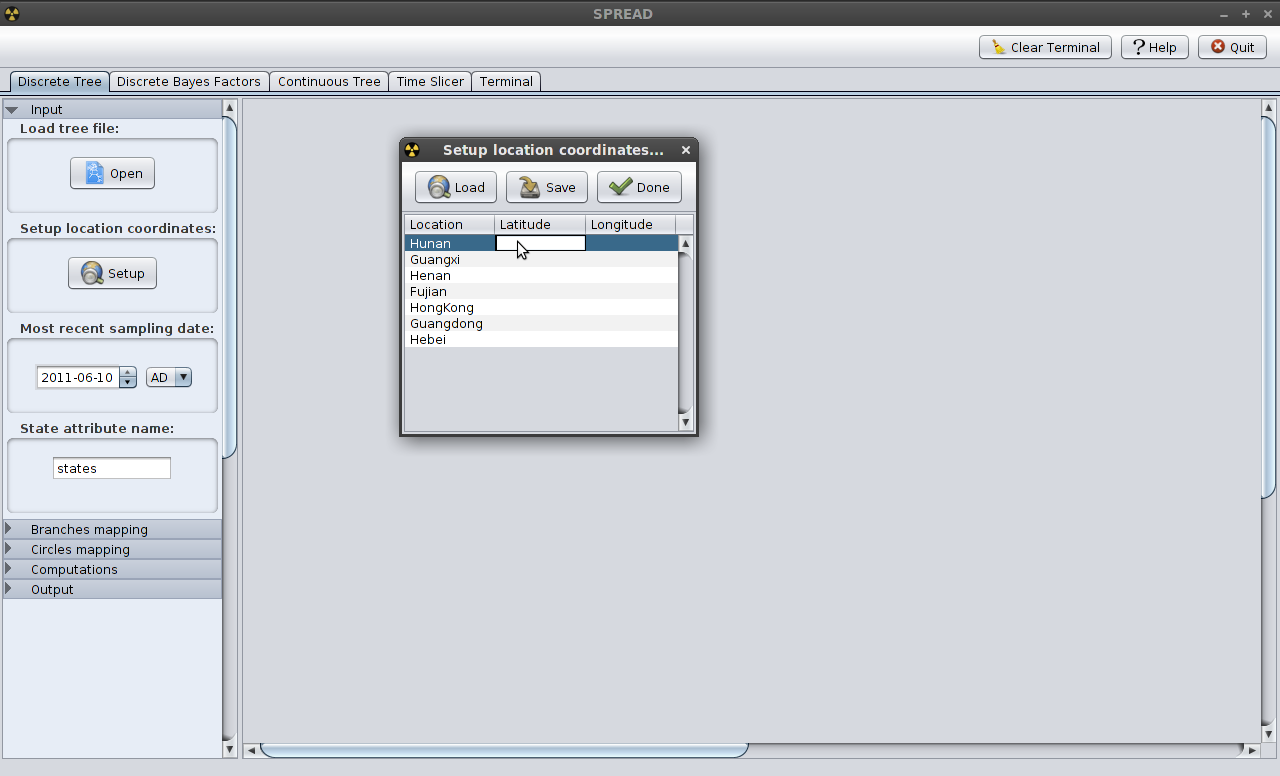
\includegraphics[scale=0.25]{fig003}
\caption{Location coordinates editor.}
\label{fig:003}
\par\end{centering}
\end{figure}

Go to the Discrete Model tab and click on Setup location coordinates
button. You should see the list of discrete locations parsed from
your tree. Click on the appropriate fields and fill them with latitude
and longitude coordinates. After you finished editing the file save
it and load it by clicking on Done button. Alternatively use the Load
button and navigate to your previously prepared location coordinates
file to load it. 

In either case when you click on Done button the Terminal tab should
show You how many discrete locations have been read by Spread, with
their names and corresponding latitude and longitude coordinates.
If you forgot to save the edited file You can still copy and paste
this output.

\begin{figure}[H]
\begin{centering}
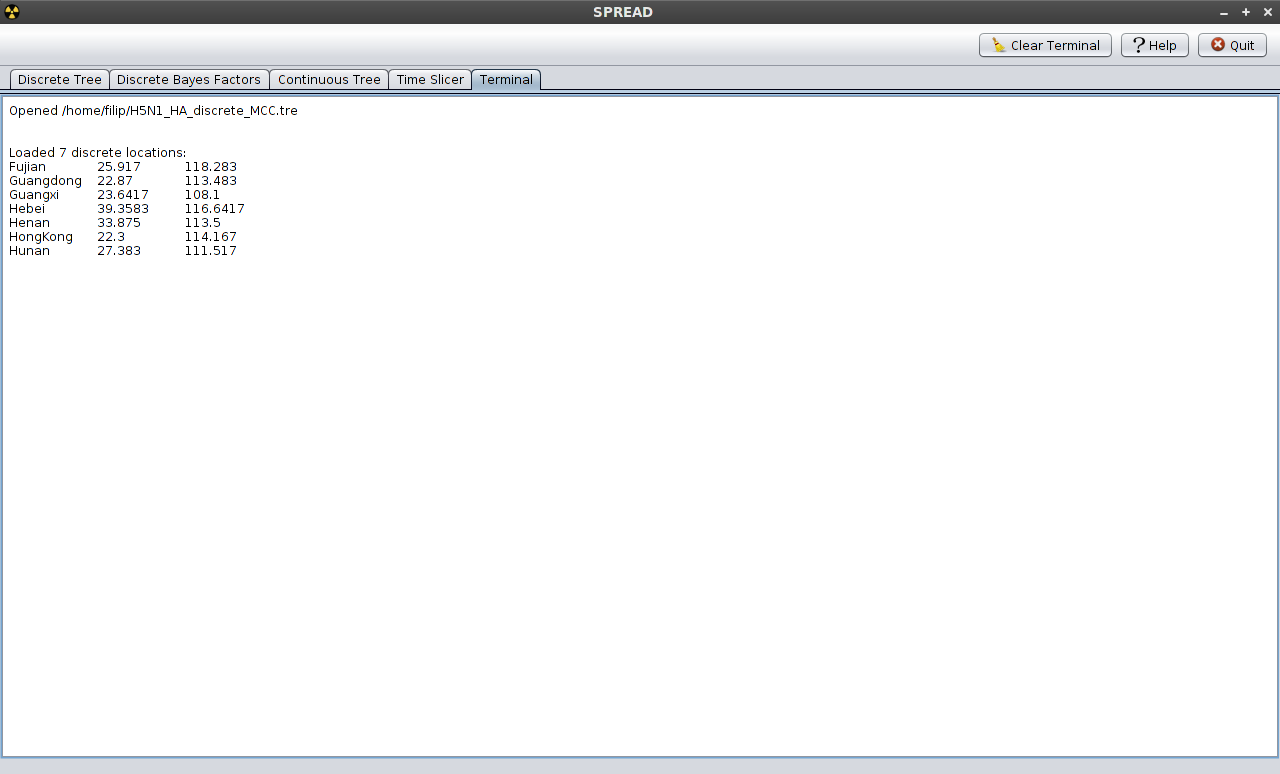
\includegraphics[scale=0.25]{fig0003}
\caption{Terminal output.}
\label{fig:0003}
\par\end{centering}
\end{figure}

\subsection{Setting the visualisation attributes}

Now that your data is loaded, you can start setting the attributes.

\begin{itemize}
\item \textbf{Most recent sampling date} (mrsd) is specified in YYYY-MM-DD
format. If You know only the year set it to the last day of the previous
year. Use the spinner to operate Year, Month and Day fields. You can
also choose whether the date is in our era (AD), or not (BC).
\item \textbf{State attribute name} is the name of tree nodes discrete locations
attribute. Common names include \textsl{state} or \textsl{states}.
Specify it accordingly, otherwise Spread would be unable to parse
the data correctly. If in doubt you can always open your tree in a
text editor and check for the attribute name. H5N1 analysis uses the
default name. 
\item \textbf{Branches color mapping} allows you to setup the minimal and
maximal colors of the plotted lines. Spread will map the node heigth
values of the MCC tree to the colors in between the specified maximal
and minimal boundary. Set both mappings to the same color if you want
no mapping assigned.
\item Adjust the size of lines using the \textbf{Branches width} slider.
\item \textbf{Circles color mapping} allows you to setup the minimal and
maximal colors of the plotted circular polygons. Those polygons will
have their colors mapped accordingly to the number of lineages holding
the discrete state at the given time (interval). You can choose the
beginning and the end values of those color mappings, by specifying
RGB, HSB opacity and brightness values.
\item The radius of circular polygons represents the number of lineages
holding the discrete state at a given time. The default value of 100
times the square root of the number of lineages can be multiplied
by a choosen constant using \textbf{Circles radius multiplier}.
\item \textbf{Number of intervals} specifies into how many intervals your
MCC tree timeline (time from tree root until the most recent sampling
date) will be cutted into. 100 intervals is a good default value for
most applications.
\item \textbf{Maximal altitude mapping} refers to the KML output. Spread
will map the geographic distances between discrete locations to the
altitude of the lines connecting them, giving higher altitudes to
the distant ones and lower altitudes to the ones lying close to each
other. Changing this attribute will modify the upper boundary of the
mapping. If you set it to 0 all lines will be flat.
\item \textbf{KML name} field allows you to specify the name of the output
file.
\end{itemize}


\begin{figure}[H]
\begin{centering}
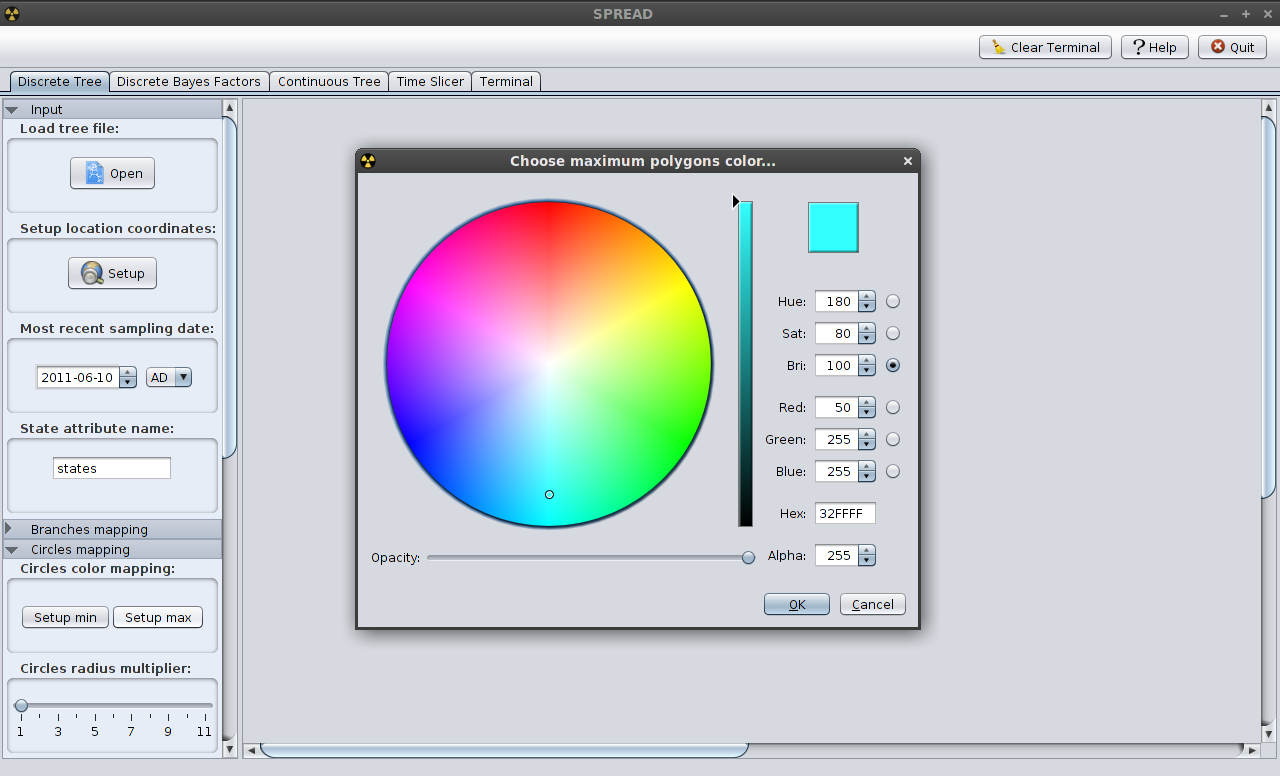
\includegraphics[scale=0.25]{fig03}
\caption{Color chooser.}
\label{fig:03}
\par\end{centering}
\end{figure}


\subsection{Generating the visualisations}

Once you're satisfied with the specified attributes click on Generate
KML button to generate output for viewing in virtual globe software.
If everything went fine you should see a message in Terminal tab indicating
how long did it take for Spread to generate the file. If something
went wrong Spread will also show a warning or an error message there.


\begin{figure}[H]
\begin{centering}
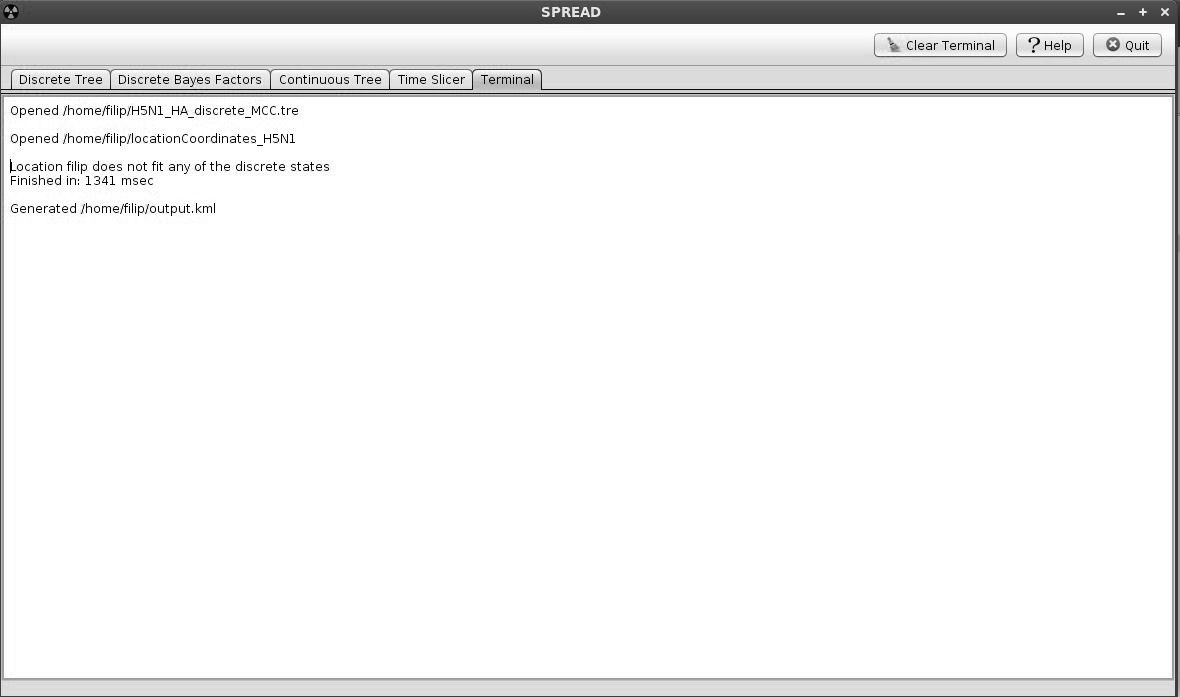
\includegraphics[scale=0.25]{fig04}
\caption{Message in Terminal.}
\label{fig:04}
\par\end{centering}
\end{figure}

The visualisation once opened for viewing in Google Earth (GE) will
have a slider indicating the time component of the phylogeny. Clicking
on the play button starts an animation of the viral diffusion over
time. 

Click on Plot map button in Spread menu to view the visualisation
in the inner Spread map. 


\begin{figure}[H]
\begin{centering}
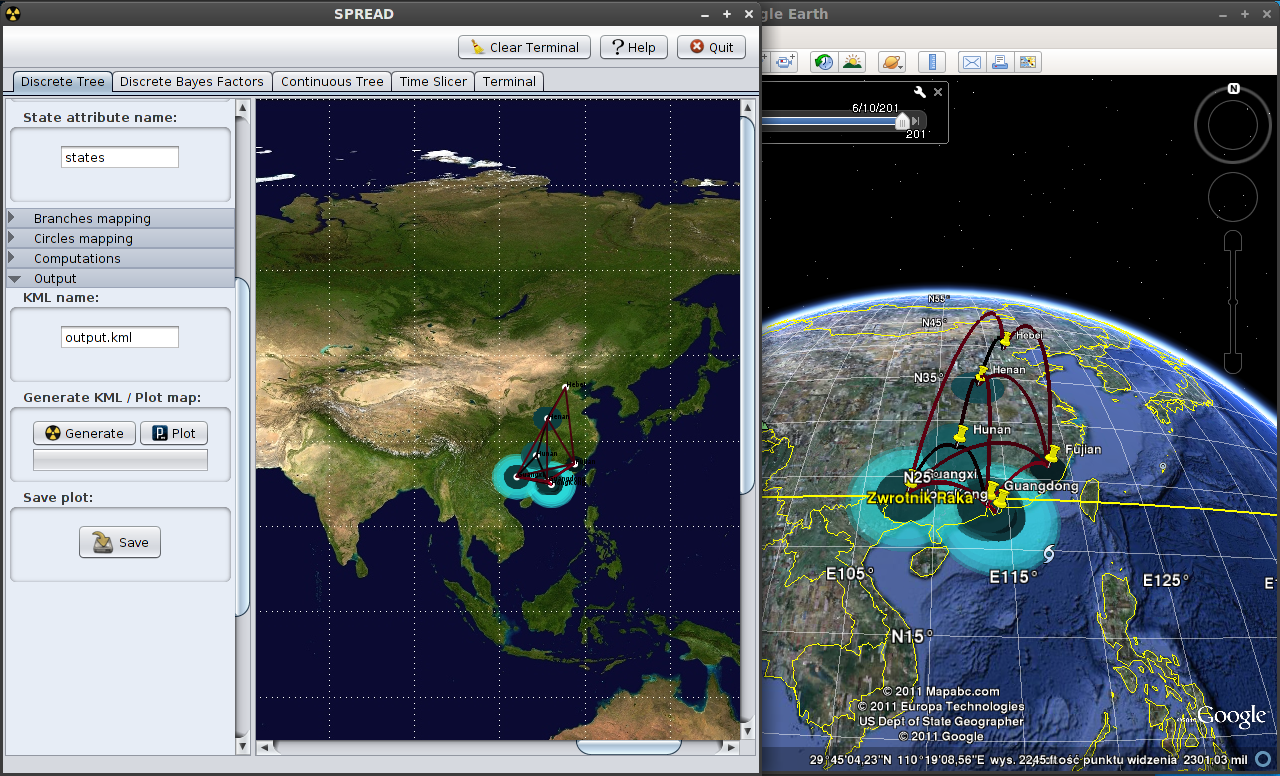
\includegraphics[scale=0.25]{H5N1_discrete_vis}
\caption{Screenshot of the Spread output.}
\label{fig:05}
\par\end{centering}
\end{figure}

\section{Identifying well supported rates using Bayes factors test}

This tutorial assumes the user has generated a BEAST log file with
rate indicators as described in Bayesian stochastic search variable
selection (BSSVS) procedure, as described here:

\url{http://beast.bio.ed.ac.uk/BSSVS} 

\noindent
The test aims at identifying frequently invoked rates to explain the
diffusion process and visualize them in virtual globe software or
using Spread own map. 

\noindent
The log file used in this example can be accessed from here:

\url{http://www.kuleuven.be/aidslab/phylogeography/SPREAD_files/H5N1_HA_discrete_rateMatrix.log}

\noindent
The location coordinates file can be downloaded using the following
url: 

\url{http://www.kuleuven.be/aidslab/phylogeography/SPREAD_files/locationCoordinates_H5N1.txt}.


\subsection{Loading the data}

Go to the Rate Indicator BF tab and load your log using proper button
and a supplied chooser, to navigate to the directory containing your
log file. 

\begin{figure}[H]
\begin{centering}
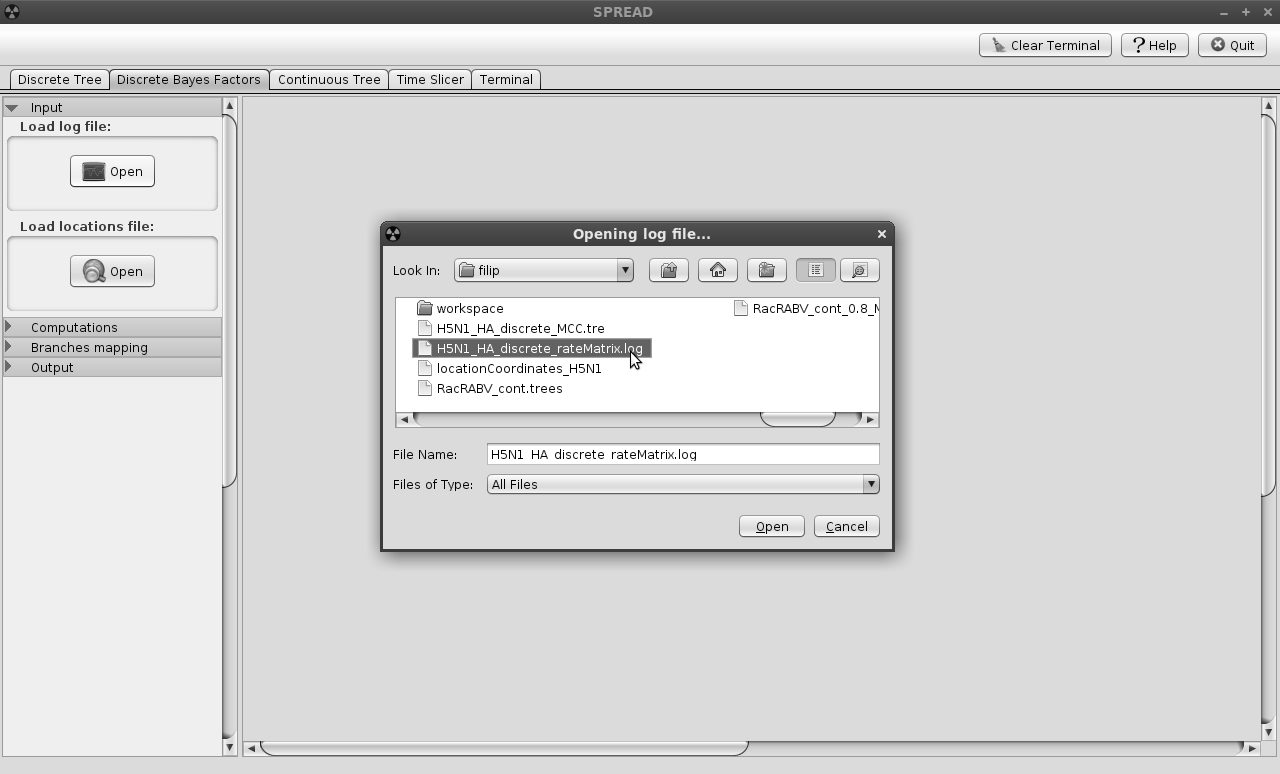
\includegraphics[scale=0.25]{fig06}
\caption{Loading the log file.}
\label{fig:06}
\par\end{centering}
\end{figure}

To analyze the results in the log file we will need a tab delimited
file with location names and their latitude and longitude coordinates.
For H5N1 analysis example this file should look like this:

\begin{lyxcode}
Fujian~25.917~118.283

Guangdong~22.87~113.483

Guangxi~23.6417~108.1

Hebei~39.3583~116.6417

Henan~33.875~113.5

HongKong~22.3~114.167

Hunan~27.383~111.517
\end{lyxcode}

You can either use the location coordinates editor to prepare it,
or load a previously saved file. In either case when you click on
Done button the Terminal tab should show you how many discrete locations
have been read by Spread, with their names and corresponding latitude
and longitude coordinates. If you forgot to save the edited file you
can still copy and paste this output.

\begin{figure}[H]
\begin{centering}
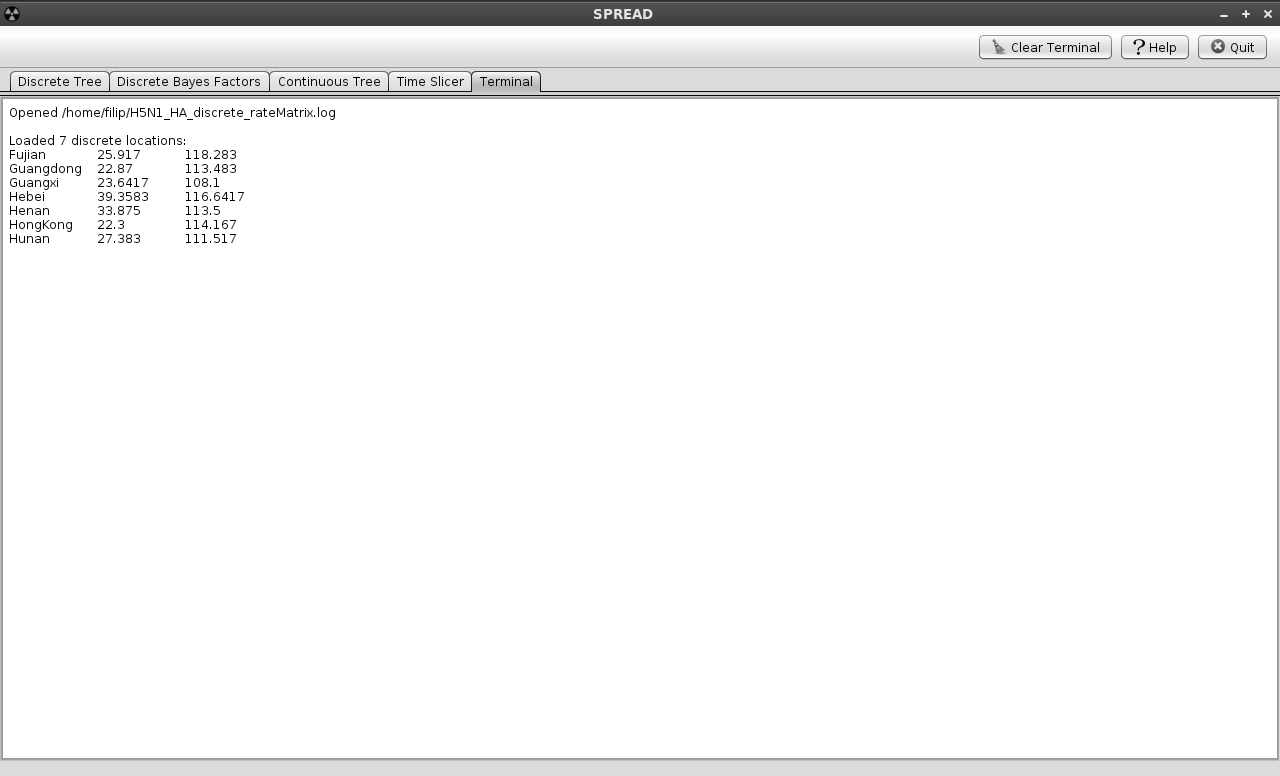
\includegraphics[scale=0.25]{fig006}
\caption{Terminal output.}
\label{fig:006}
\par\end{centering}
\end{figure}

\subsection{Setting the visualisation attributes}

Now that your data is loaded, you can start setting the attributes.

\begin{itemize}
\item Use \textbf{Specify burn-in} slider to set how many initial samped
values should be discarded from the analysis. The default value of
10\% should be sufficient for most of the analysis.
\item \textbf{Poisson prior mean/offset} specifies the mean of the (truncated)
Poisson prior (the default value is $log(2)$ unless specified otherwise)
and the offset of the (truncated) Poisson prior (the default is the
number of locations - 1 unless specified otherwise).
\item \textbf{Bayes factor cut-off} specifies the Bayes factor values above
which we consider rates to be well supported (only those rates will
be visualised). For H5N1 analysis the default cut-off of 3.0 is sufficient. 
\item \textbf{Rates color mapping} allows you to setup the minimal and maximal
colors of the plotted lines. Spread will map the log of bayes factors
values to the colors in between the specified maximal and minimal
boundary.
\item Adjust the size of lines using the \textbf{Rates width} slider.
\item \textbf{Number of intervals} is a purely technical attribute and specifies
of how many line segments your rate lines will consist of, setting
this number too small can result in crude looking lines. We suggest
leaving the default value of 100.
\item \textbf{Maximal altitude mapping} refers to the KML output. Spread
will map the geographic distances between discrete locations to the
altitude of the lines connecting them, giving higher altitudes to
the distant ones and lower altitudes to the ones lying close to each
other. Changing this attribute will modify the upper boundary of the
mapping. If you set it to 0 all lines will be flat.
\item \textbf{KML name} field allows you to specify the name of the output
file.
\end{itemize}

\subsection{Generating the visualisations}

Once you're happy with the specified plotting attributes click on
the Generate KML button. Spread will now output the kml file in its
current working directory, you can view this file using google Earth
or any other software capable of reading the format. You can also
see the visualisation using Spreads own map by clicking the Plot button.

\begin{figure}[H]
\begin{centering}
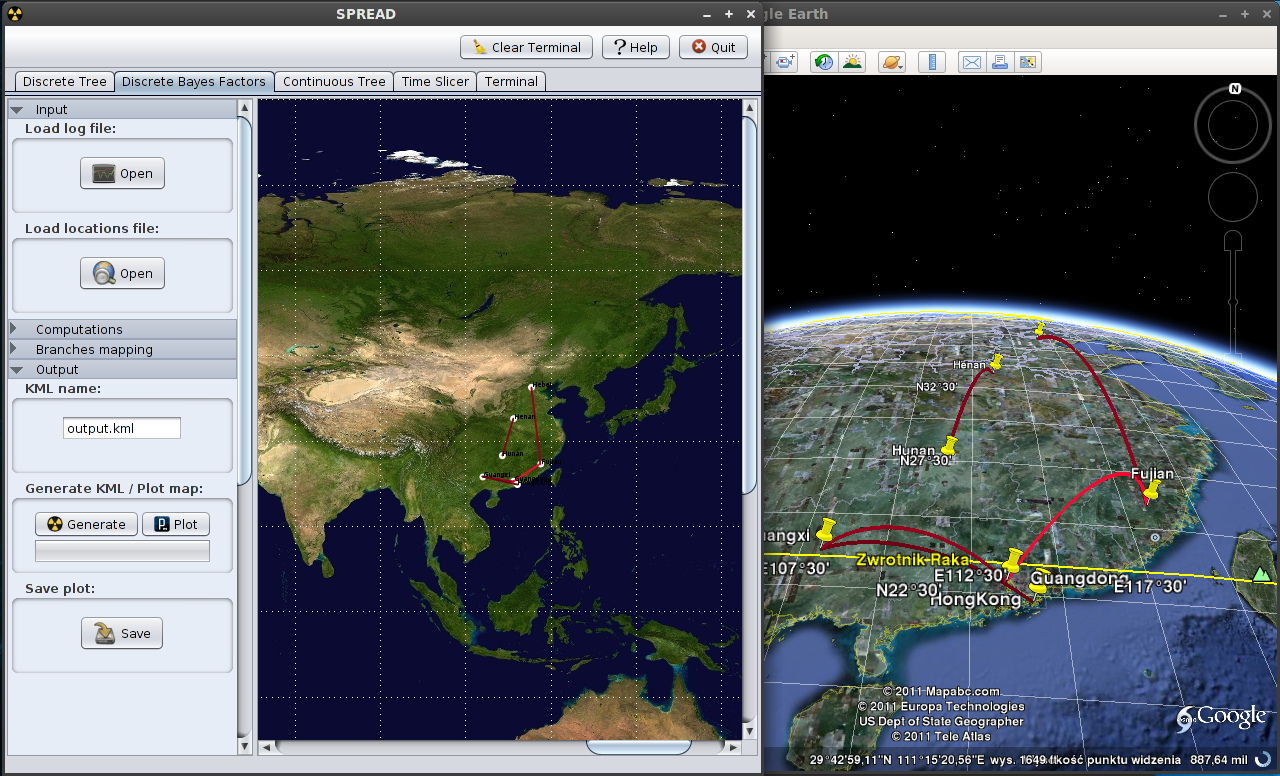
\includegraphics[scale=0.25]{H5N1_bf_vis}
\caption{Generated visualisations.}
\label{fig:07}
\par\end{centering}
\end{figure}

Both plotting and generating kml output file should result in a lists
with the rates yielding a bayes factor above the specified cut-off
to be printed in the terminal tab. You copy and paste this output
for later use. The rates are by default sorted in ascending order.


\begin{figure}[H]
\begin{centering}
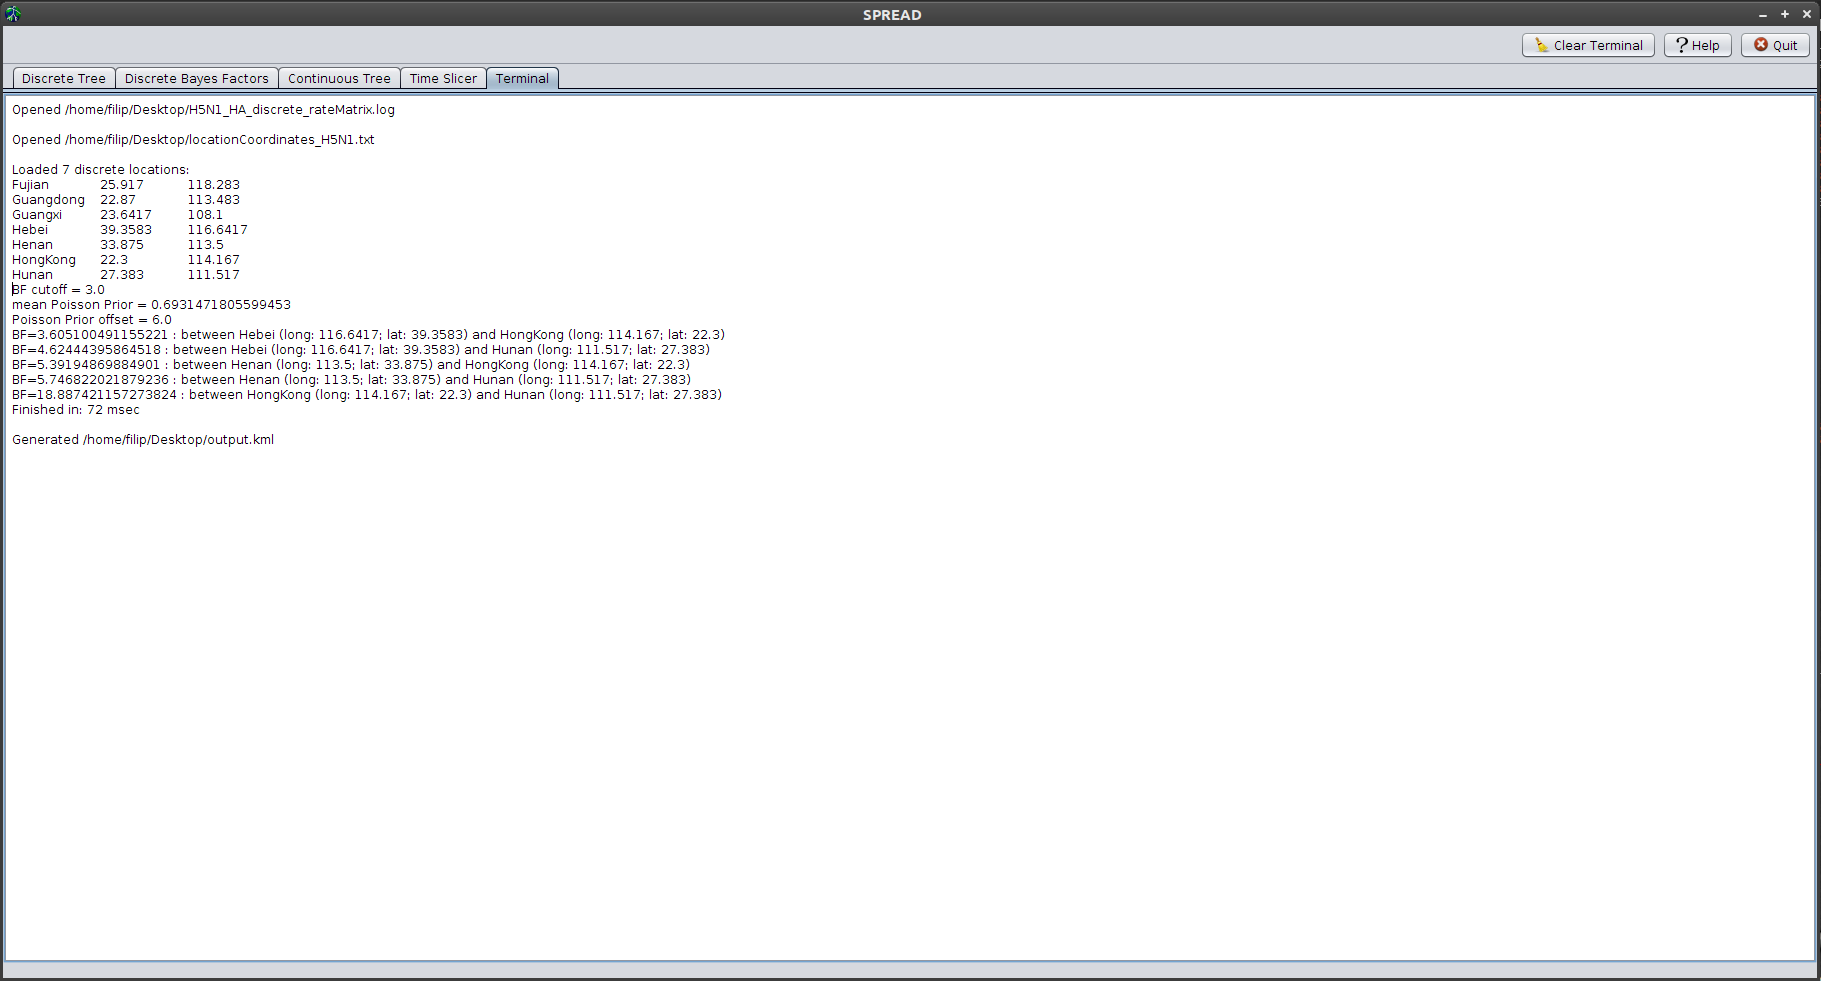
\includegraphics[scale=0.2]{fig08}
\caption{Terminal tab output.}
\label{fig:08}
\par\end{centering}
\end{figure}

\section{Visualising a continuous MCC tree}

This tutorial assumes the user has set up a BEAST phylogeographic
analysis in continuous space and generated a Maximum Clade Credibility
(MCC) tree using TreeAnnotator. Good tutorial on neccessary steps
can be found here:

\url{http://beast.bio.ed.ac.uk/Continuous_phylogeographic_analysis}

\noindent
This visualisation aims at projecting the MCC tree on the grid of
geographical coordinates, with polygons representating the uncertainty
in location coordinates and considers raccoon rabies diffusion in
north-eastern United States. 
The example tree file used in the presented analysis can be accessed
from here:

\url{http://www.kuleuven.be/aidslab/phylogeography/SPREAD_files/RacRABV_cont_0.8_MCC_snyder.tre}


\subsection{Loading the data}

Click on Continous model tab and load your MCC tree into Spread. If
you now open the Terminal tab Spread will show message with path to
your file, indicating it has set the working directory to the one
your file is in (generated output will go there).

\begin{figure}[H]
\begin{centering}
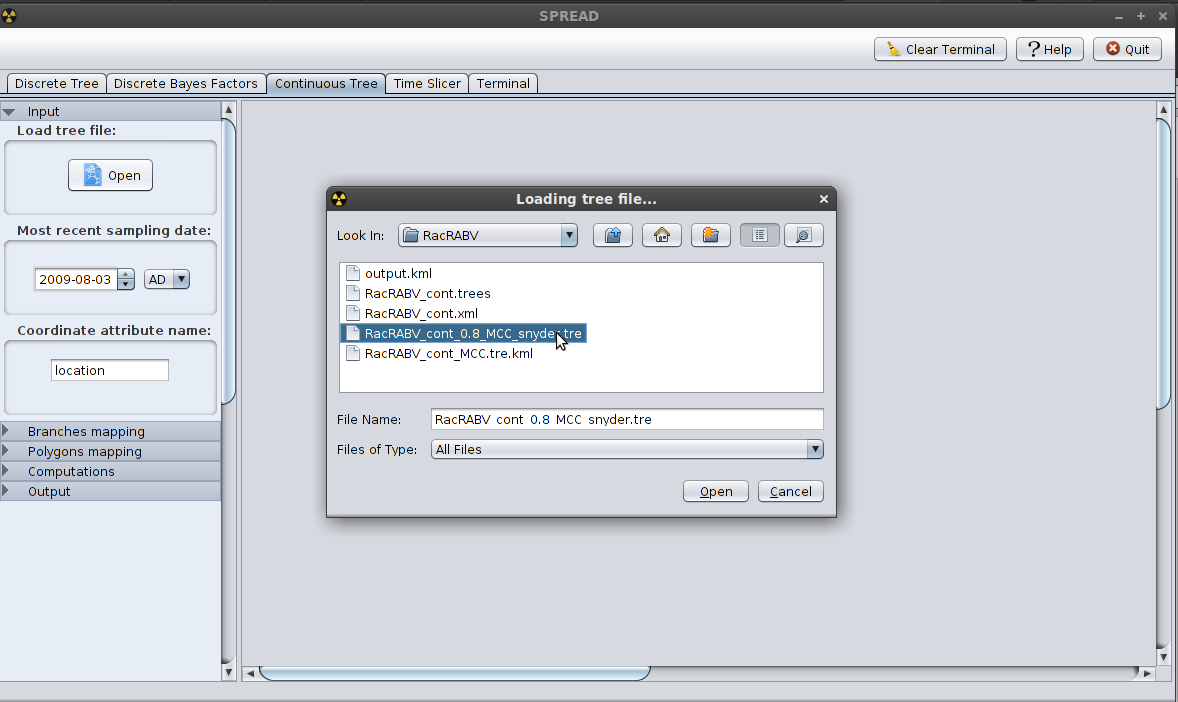
\includegraphics[scale=0.25]{fig09}
\caption{Loading tree file.}
\label{fig:09}
\par\end{centering}
\end{figure}

\subsection{Setting the visualisation attributes}

\begin{itemize}
\item \textbf{Most recent sampling date} (mrsd) is specified in YYYY-MM-DD
format. If you know only the year set it to the last day of the previous
year. Use the spinner to operate Year, Month and Day fields. You can
also choose whether the date is in our era (AD), or not (BC). 
\item \textbf{Coordinate attribute name} is the name of tree nodes coordinate
attribute. Common names include \textsl{location} or \textsl{trait}.
Specify it accordingly, otherwise Spread would be unable to parse
the data correctly. If in doubt you can always open your tree in a
text editor and check what's that attribute name. Racoon rabies data
that we will use in this tutorial uses \textsl{location }as the attribute
name.
\item \textbf{Branches color mapping} allows you to setup the minimal and
maximal color values of the plotted lines. Spread will map the node
heigth values of the MCC tree to the colors in between the specified
set, what results in the continuous color gradient on your visualisation.
\item Adjust the size of branch lines using the \textbf{Branches width}
slider.
\item \textbf{Maximal altitude mapping} refers to the KML output. Spread
will map the geographic distances between discrete locations to the
altitude of the lines connecting them, giving higher altitudes to
the distant ones and lower altitudes to the ones lying close to each
other. Changing this attribute will modify the upper boundary of the
mapping. If you set it to 0 all lines will be flat.
\item \textbf{Polygons color mapping} allows you to setup the minimal and
maximal colors of the plotted polygons. Those polygons will have their
colors mapped accordingly to the relative time of the dispersal pattern.
You can choose the beginning and the end values of those color mappings,
by specifying RGB, HSB, opacity and brightness values.
\item \textbf{Number of intervals} specifies into how many intervals your
timeline (time from tree root until the most recent sampling date)
should be cut into. 100 intervals is a good default value for most
visualisations.
\item \textbf{KML name} field allows you to specify the name of the output
file.
\end{itemize}

\subsection{Generating the visualisations}

Once you're satisfied with the specified attributes click on Generate
KML button to generate output for viewing in virtual globe software.
If everything went fine you should see a message in the Terminal tab
indicating how long did it take for Spread to generate the file. The
generated output can now be opened for viewing in Google Earth. Once
opened in GE visualisation will have a slider indicating the time
component of the tree. Clicking on the play button starts an animation
of the viral diffusion through time. Click on Plot map button in Spread
menu to view the visualisation in the inner Spread map.

\begin{figure}[H]
\begin{centering}
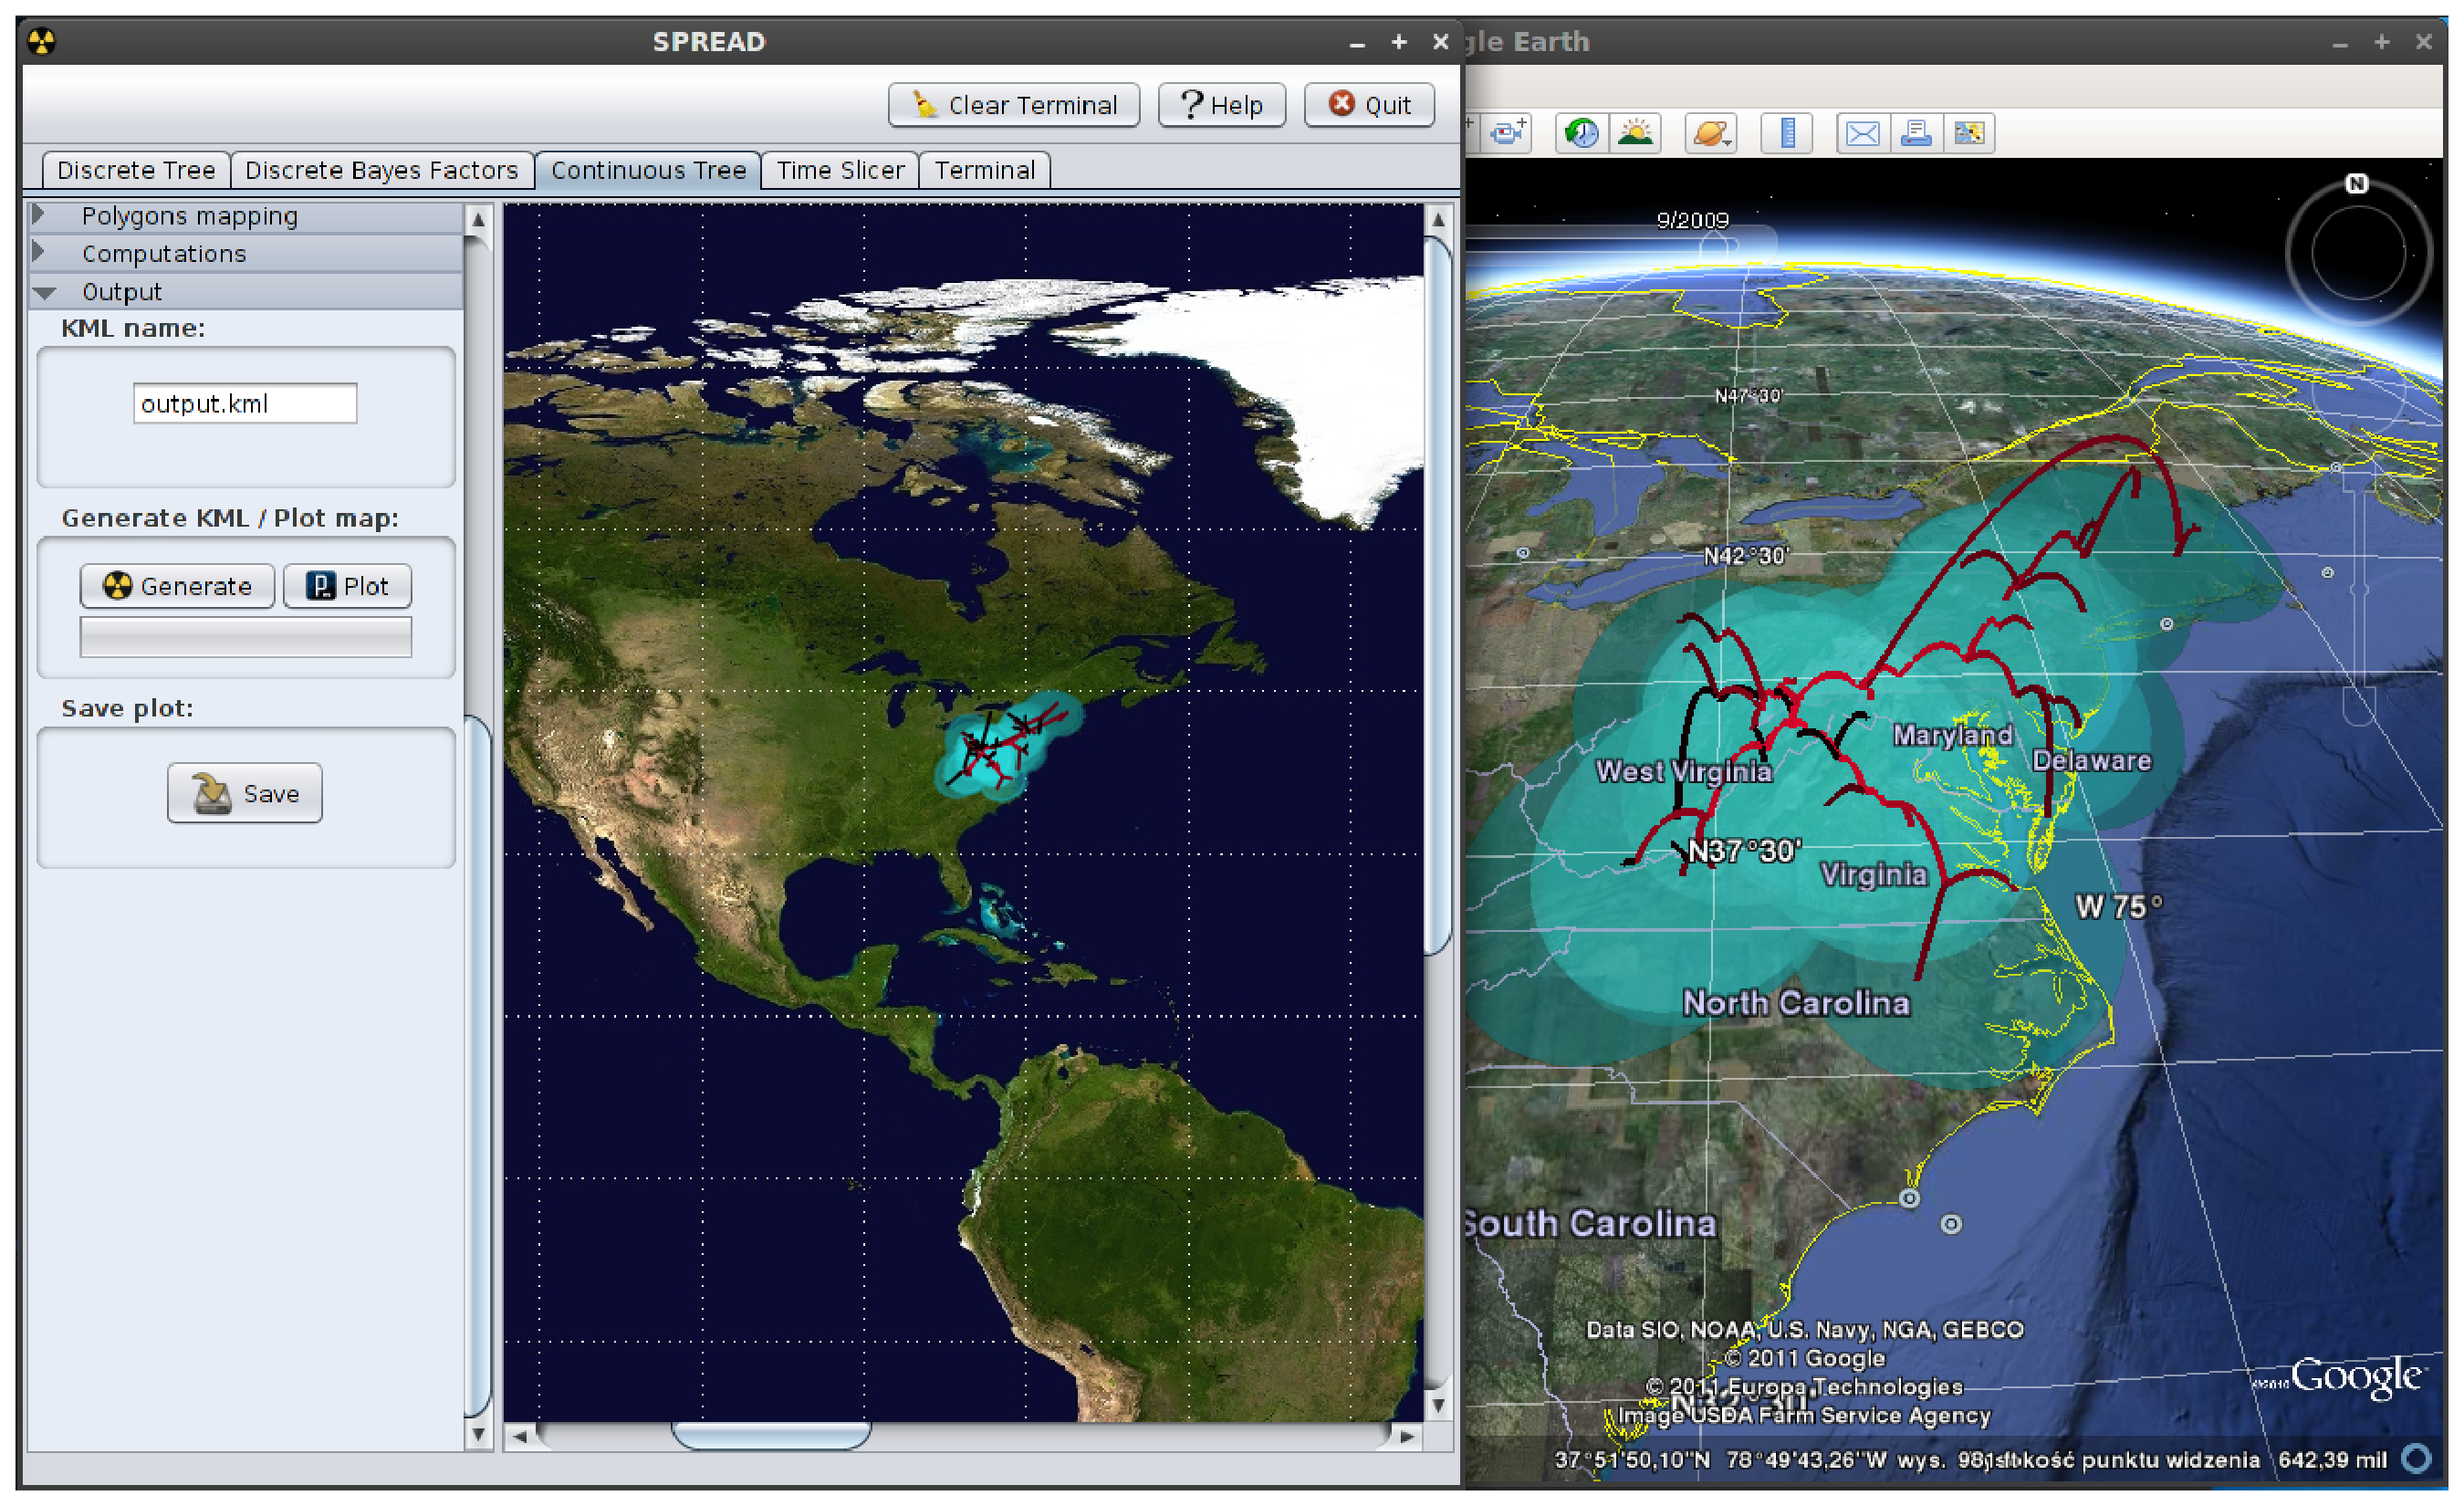
\includegraphics[scale=0.25]{RacRABV_cont_vis}
\caption{TScreenshot of the Spread output.}
\label{fig:RacRABV_cont_vis}
\par\end{centering}
\end{figure}

\section{Summarising full posterior distribution}

This tutorial assumes the user has set up a BEAST phylogeographic
analysis in continuous space and generated a trees file and an MCC
tree file using TreeAnnotator. Good tutorial on neccessary steps can
be found here:

\url{http://beast.bio.ed.ac.uk/Continuous_phylogeographic_analysis}

\noindent
This analysis allows one to summarise and visualise full posterior
distribution of the trees obtained in continuous phylogeographic analysis.
To achieve this Spread creates a time line according to the MCC tree
length, slices through each phylogeny at a particular points in time,
imputes the unobserved descendant locations for those time points
and contoures them by creating polygons, a natural representation
of the uncertainty in these inferences. In this template we also visualise
the MCC tree which gave rise to the time slices by drawing it's branches.

Since Spread version 1.0.2 user can choose to supply custom slice
heights instead of automatically defining them according to the MCC
tree. This can be done by choosing appropriate analysis type and then
loading text file with the custom slice times.

\begin{figure}[H]
\begin{centering}
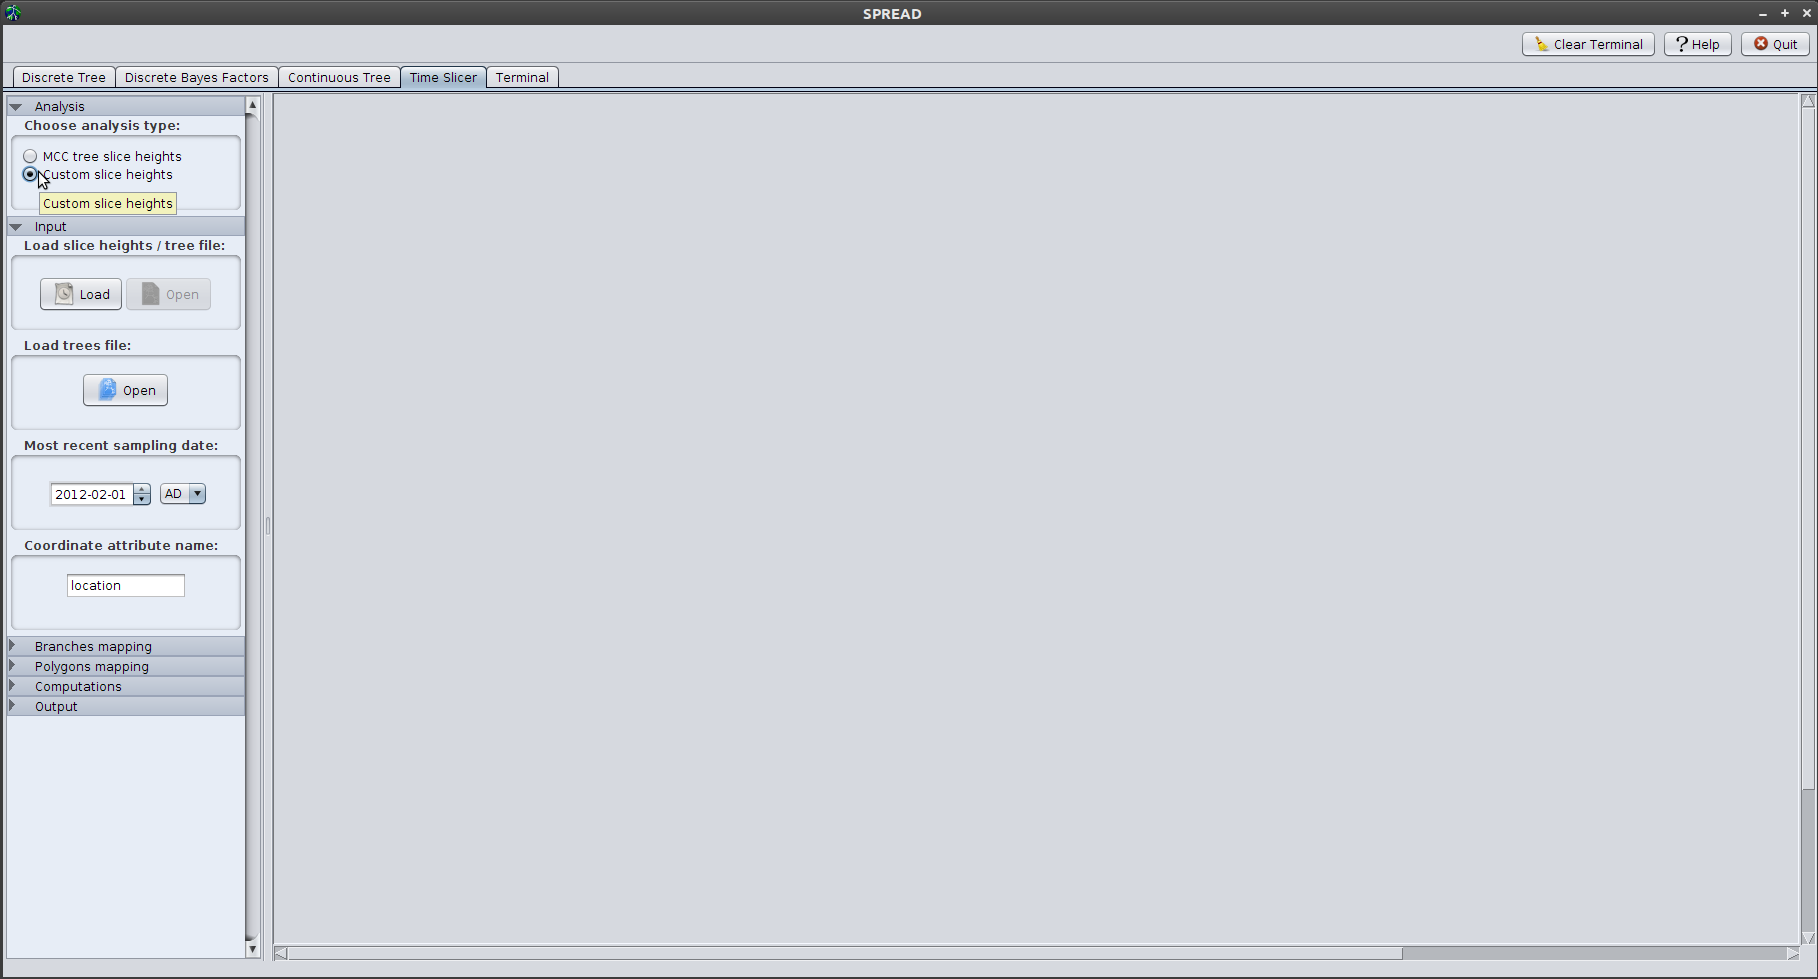
\includegraphics[scale=0.2]{fig10}
\caption{Choosing analysis type.}
\label{fig:10}
\par\end{centering}
\end{figure}

We will use the same racoon rabies data as in the continuous tree
visualisation. The tree files used in this analysis can be downloaded
from:

\url{http://www.kuleuven.be/aidslab/phylogeography/SPREAD_files/RacRABV_cont_0.8_MCC_snyder.tre}

\noindent
and the trees file from:

\url{http://www.kuleuven.be/aidslab/phylogeography/SPREAD_files/RacRABV_cont.trees}

\noindent
Note that this analysis is much more resource-hungry and you might
want to increase the heap space availiable for the Java Virtual Machine.
This can be done by starting Spread from command line with the following
arguments: 

\begin{lyxcode}
java~-jar~-Xmx2024m~spread.jar
\end{lyxcode}

\subsection{Loading the data}

First you need to load the MCC tree that gives rise to the time intervals.
Do this using the Load tree file button. Next import the trees file
using Load trees file button. Once you're done start setting the appropriate
attributes.


\subsection{Setting the visualisation attributes}

Now that your data is loaded, you can start setting the plotting attributes.
Time Slicer template allows for the following options to be specified: 

\begin{itemize}
\item \textbf{Most recent sampling date }(mrsd) is specied in YYYY-MM-DD
format. Use the spinner to operate Year, Month and Day fields. You
can also choose whether the date is in our era (AD), or not (BC). 
\item \textbf{Coordinate attribute name} is the name of tree nodes coordinate
attribute. Specify it correctly, otherwise Spread would be unable
to parse the data correctly, what results in error message.
\item \textbf{Branches color mapping} allows you to setup the minimal and
maximal color values of the plotted lines. Spread will map the node
heigth values of the MCC tree to the colors in between the specified
maximal and minimal boundary what results in the continuous color
gradient for those values.
\item \textbf{Branches width} slider allows to adjust the size of branch
lines.
\item \textbf{Maximal altitude mapping} refers to the KML output. Spread
will map the geographic distances between discrete locations to the
altitude of the lines connecting them, giving higher altitudes to
the distant ones and lower altitudes to the ones lying close to each
other. Changing this attribute will modify the upper boundary of the
mapping. If you set it to 0 all lines will be flat.
\item \textbf{Polygons color mapping} allows you to setup the minimal and
maximal colors of the plotted polygons. Those polygons will have their
colors mapped accordingly to the relative time of the dispersal pattern.
You can choose the beginning and the end values of those color mappings,
by specifying RGB, HSB opacity and brightness values.
\item You can choose the \textbf{Use true noise} checkbox if you wish to
interpolate between the imputed locations. You then have to specify
the appropriate \textbf{Rate attribute name} and \textbf{Precision
attribute name}, using the text fields.
\item \textbf{Specify burn-in} is the field in which you let the Spread
know how many initial trees should be discarded from the analysis. 
\item Use highest posterior density \textbf{(HPD}) field to specify the
level of the kernel density estimation. Common values used are 0.8,
0.95 and 0.99.
\item \textbf{Number of intervals} specifies into how many intervals your
timeline (time from the root of the phylogeny until the most recent
sampling date) should be cut into. 100 intervals is a good default
value for most visualisations.
\item \textbf{Grid size} slider lets you adjust the number of points used
in contouring. In general the larger the value the smoother the generated
polygons will be, however the analysis also gets more computationally
involved as this value increases.
\item \textbf{KML name} field allows you to specify the name of the output
file.
\end{itemize}

\subsection{Generating the visualisations}

When you are satisfied with specified attributes click on the Generate
KML button to export the results to keyhole markup language or the
Plot button to visualise them on a map. Depending on the size of your
data the analysis might take some time. You can observe the progress
and errors if any, in the Terminal tab.

Once Spread is done you can open the resulting kml file in the virtual
globe software and animate the spatial diffusion over time.

\begin{figure}[H]
\begin{centering}
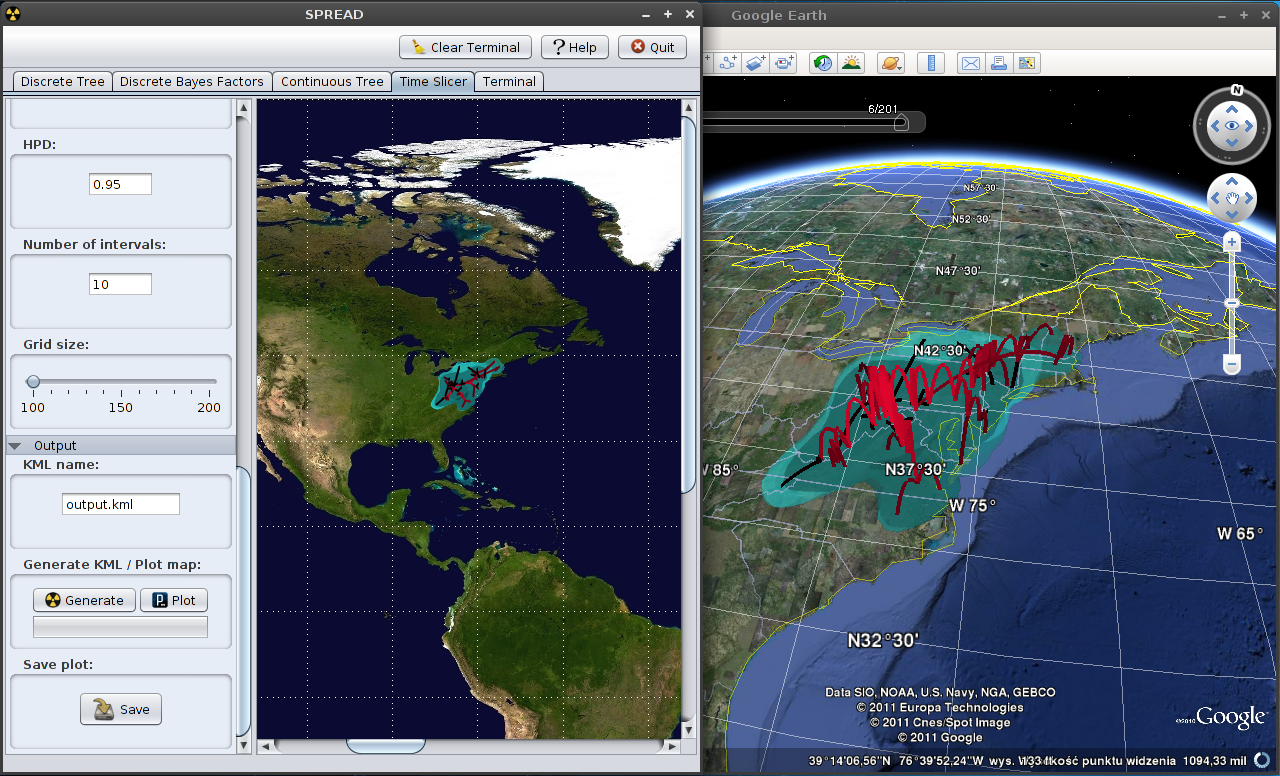
\includegraphics[scale=0.25]{RacRABV_Time_Slicer_vis}
\caption{Terminal tab output.}
\label{fig:12}
\par\end{centering}
\end{figure}

\section{Tips \& tricks}

For some Mac users Spread refuses to generate KML output of the Bayes
factors test, even though it claims to have done so in the Terminal
output. This problem can be fixed by starting Spread with more memory
availliable. To do so start Spread from command line with the following
arguments: 

\begin{lyxcode}
java~-jar~-Xmx2024m~spread.jar
\end{lyxcode}